\documentclass[11pt,a4paper]{article}

\usepackage[T1]{fontenc}
\usepackage{lmodern}
\usepackage[english]{babel}
\usepackage[margin=2.4cm]{geometry}
\usepackage{microtype}
\usepackage{setspace}
\usepackage{amsmath}
\usepackage{graphicx}
\usepackage{booktabs}
\usepackage{tabularx}
\usepackage{caption}
\usepackage{float}
\usepackage{xcolor}
\usepackage[authoryear,round]{natbib}
\usepackage[hyphens]{url}
\usepackage[colorlinks=true,linkcolor=black,citecolor=blue!50!black,urlcolor=blue!50!black]{hyperref}

\graphicspath{{../figures/Gabri/}}
\captionsetup{font=small,labelfont=bf}
\setstretch{1.08}
\Urlmuskip=0mu plus 1mu\relax
\setlength{\parskip}{0.4em}
\setlength{\parindent}{0pt}

\title{\textbf{Heat and drought in Catalonia:\\ what they do to electricity use, olive oil prices\\ and access to cooling}}
\author{Gabriel Albasini Garaulet\\[2pt]
\small MSc in Physics of Complex Systems and Biophysics, Universitat de Barcelona}
\date{\small Course project, \emph{Analysis and Visualization of Big Data} (2026/27)\\ November 2026}

\begin{document}
\maketitle

\begin{abstract}
\noindent
We asked three plain questions about heat and drought in Catalonia and answered them with open data. How much more electricity does the region use on hot and on cold days? When the 2022--2024 drought cut hydropower, who filled the gap? Do dry years raise olive oil prices? We added a fourth question for Barcelona: can residents reach a climate shelter on foot, whatever their income? Electricity demand has a comfort zone of about 17--22\,$^\circ$C. Each degree above it adds 4.2\,GWh per day, and each degree below adds 2.9\,GWh. Hydropower follows rain in the Pyrenees, not the reservoirs near Barcelona, and most of the missing electricity in 2023 came through imports, not from gas plants. Olive oil prices relate only weakly to rain in Andalusia ($r=-0.42$, 23 years). In Barcelona, 99.5\% of residents live within 800\,m of a climate shelter, and poorer districts are not worse served. We expected four things; only one held, and only weakly. We explain why the others failed.
\end{abstract}

\section{Introduction}

Droughts and heat waves are easy to see on a weather map. Their effects on everyday life are harder to see, because they hide in electricity use, in supermarket prices and in the places where people can cool down. This paper follows those three traces in Catalonia and Barcelona, using only open data.

The work is one part of a group project on climate extremes in Catalonia, and it covers the economic and social side. We started with four expectations:
\begin{enumerate}
\item[\textbf{H1}] Electricity demand rises more steeply with cold than with heat.
\item[\textbf{H2}] When hydropower fell during the 2022--2024 drought, gas-fired plants made up the difference.
\item[\textbf{H3}] Dry years push up olive oil prices, and rain in Andalusia (Ja\'en and C\'ordoba, a major olive-growing area) explains the price better than rain in Catalonia.
\item[\textbf{H4}] Poorer neighbourhoods of Barcelona have fewer climate shelters within walking distance.
\end{enumerate}
We tested each one and report what the data say, including where they disagree with us.

\section{Data and methods}

\subsection{Data}

All data are open and come from public sources (Table~\ref{tab:data}). We downloaded them through their APIs and cached the raw files, so every figure can be rebuilt from the code in the project repository.

\begin{table}[H]
\centering
\small
\begin{tabularx}{\linewidth}{@{}l X l@{}}
\toprule
Topic & Data and source & Period\\
\midrule
Electricity demand & Daily demand in Catalonia, in MWh \citep{demand} & 2019--2025\\
Generation & Monthly generation by technology, Catalonia \citep{redata} & 2019--2025\\
Net imports & Monthly electricity exchange balance, Catalan energy indicators \citep{indicators} & 2019--2025\\
Temperature, rain & Daily data from XEMA weather stations \citep{xema} & 2002--2025\\
Rain in Andalusia & Daily rain at two grid points near Ja\'en and C\'ordoba, from an ERA5-based reanalysis \citep{openmeteo,era5} & 2002--2025\\
Reservoirs & Daily volume of the nine reservoirs of the Conques Internes basin \citep{aca} & 2019--2025\\
Prices & Monthly consumer price index (CPI) by product \citep{ine} & 2002--2025\\
Barcelona & Income per person, population by age, census sections, climate shelters, vulnerability to heat \citep{bcn} & 2015--2026\\
\bottomrule
\end{tabularx}
\caption{Data used in this study.}
\label{tab:data}
\end{table}

\subsection{Electricity demand and temperature}

We compared daily electricity demand with the daily mean temperature at the Raval station in central Barcelona (33\,m above sea level). To avoid distortions, we kept weekdays from 2022 to 2025 and dropped Catalan public holidays, August, and 28 April 2025, an outlier of only 69\,GWh that coincides with the Iberian blackout. That left 912 days. We described demand $D$ as a flat comfort zone with a straight rise on each side:
\begin{equation}
D(T)=D_0+a_c\,\max(T_c-T,\,0)+a_h\,\max(T-T_h,\,0),
\end{equation}
where $T_c$ and $T_h$ are the cold and heat thresholds, and $a_c$ and $a_h$ are the slopes in GWh per degree. We fitted $D_0$, $a_c$ and $a_h$ by least squares and searched for the thresholds on a grid of 0.5\,$^\circ$C. We repeated the fit with two other Barcelona stations to see how much the choice of thermometer matters.

\subsection{Hydropower, rain and imports}

We compared the yearly change in generation by source with the change in net imports, which we take from the electricity exchange balance of the Catalan energy indicators. To link hydropower with water, we used two measures. The first is the volume of the nine reservoirs of the Conques Internes basin, expressed as a share of their total capacity. The second is the rain recorded by 13 XEMA valley stations in the Pyrenean comarques. For monthly comparisons we removed the seasonal cycle by subtracting the mean of the same calendar month, and we call the result an \emph{anomaly}.

\subsection{Olive oil prices and rain}

We used the annual change of the olive oil CPI in December, because the harvest runs from November to February. As the measure of drought we used the rain of the hydrological year (October to September), standardised over 2003--2025 (a $z$-score; negative means drier than average). We chose both definitions before looking at the results. We also computed lagged correlations between monthly price changes and 12-month accumulated rain anomalies, for lags of 0 to 24 months. Rain in Catalonia is the mean of ten XEMA stations in the main farming comarques. Rain in Andalusia comes from a reanalysis grid, not from stations.

\subsection{Climate shelters in Barcelona}

For each of the 1\,068 census sections we measured the share of its area lying within 400\,m and 800\,m (about 5 and 10 minutes on foot) of the nearest shelter, in a straight line, and multiplied it by the population of the section. This treats the population as spread evenly inside each section. We then summed over groups of sections. The groups are income deciles, built so that each contains about 10\% of the residents, and three classes of a heat vulnerability score from a municipal study of the 2015 heat wave. We repeated the calculation for residents aged 75 or older. Population and age data refer to 1 January 2024.

\section{Results}

\subsection{Demand: heat weighs more than cold}

Demand is lowest between 17 and 22\,$^\circ$C, at about 114\,GWh per day (Figure~\ref{fig:demand}). Above 22\,$^\circ$C, each extra degree adds 4.2\,GWh, which is 3.7\% of the base load. Below 17\,$^\circ$C, each degree adds 2.9\,GWh, or 2.5\%. The model puts demand at about 146\,GWh on a 6\,$^\circ$C day and about 152\,GWh on a 31\,$^\circ$C day. The spread around the curve is large (a residual error of 5.8\,GWh), and at the same temperature winter days use more electricity than spring days. Temperature therefore explains part of demand, not all of it.

Our expectation \textbf{H1} was wrong: the heat side is steeper. The choice of thermometer matters. The Observatori Fabra station sits at 410\,m in the Collserola hills and reads on average 2.3\,$^\circ$C cooler than the Raval station. With Fabra, the thresholds fall to 15 and 19\,$^\circ$C and the heat slope to 3.2\,GWh per degree (Table~\ref{tab:stations}). We report the Raval results because most electricity is used in the dense, urban part of the region.

\begin{figure}[t]
\centering
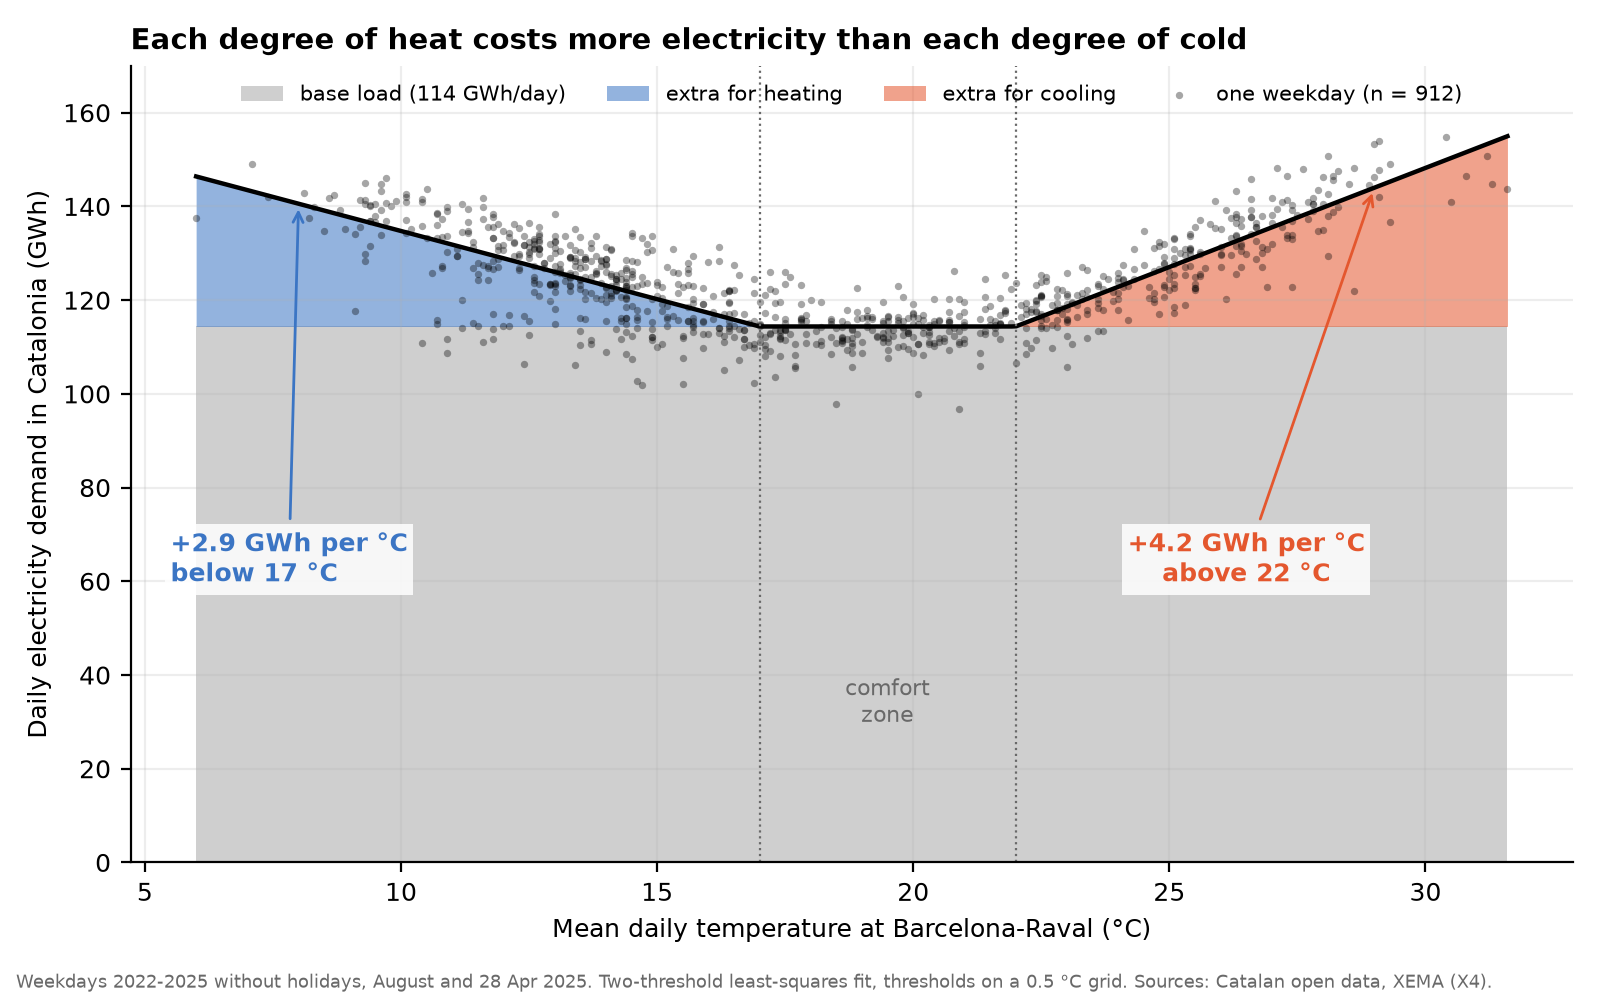
\includegraphics[width=0.72\linewidth]{idea6_demand_vs_temperature.png}
\caption{\textbf{Heat raises demand faster than cold.} Daily electricity demand in Catalonia against mean temperature at the Raval station (912 weekdays, 2022--2025). The fitted curve (black) is split into a base load (grey) and the extra demand for heating (blue) and cooling (red); the axis starts at zero, so the areas show the real size of each part.}
\label{fig:demand}
\end{figure}

\begin{table}[t]
\centering
\small
\setlength{\tabcolsep}{5pt}
\begin{tabular}{@{}lrcrrr@{}}
\toprule
Station & Alt. (m) & Thresholds ($^\circ$C) & Cold slope & Heat slope & Error (GWh)\\
\midrule
Raval (urban) & 33 & 17 / 22 & 2.91 & 4.23 & 5.80\\
Zona Universit\`aria & 82 & 17 / 21 & 2.54 & 3.90 & 5.76\\
Observatori Fabra & 410 & 15 / 19 & 2.42 & 3.22 & 6.20\\
\bottomrule
\end{tabular}
\caption{The same fit with three Barcelona stations (912 days). Thresholds are the cold and the heat threshold; slopes are in GWh per degree. Fabra is in the Collserola hills.}
\label{tab:stations}
\end{table}

\subsection{Drought and hydropower: imports filled the gap}

The reservoirs of the Conques Internes basin fell from about 95\% of capacity in spring 2020 to 15\% in February 2024. Hydropower fell too: it produced 3\,382\,GWh in 2021 and 2\,220\,GWh in 2023, which was only 5.8\% of Catalan generation. Nuclear plants supplied 59\%.

Table~\ref{tab:changes} shows who covered the loss. In 2022 the hydropower fall coincided with a jump in combined-cycle gas plants of 3\,097\,GWh. That jump belongs to the gas market. Spain capped the gas price used for power from June 2022, gas use for power rose by 52.7\% and exports to France increased \citep{cgep}. In 2023, hydropower fell by 458\,GWh, but combined-cycle output fell as well (by 2\,014\,GWh), as did nuclear output (by 1\,437\,GWh). Net imports rose by 2\,575\,GWh, from 3\,098 to 5\,672\,GWh, about 13\% of demand. So \textbf{H2} fails: the gas plants did not step in. Local generation shrank and imports grew.

\begin{table}[t]
\centering
\small
\begin{tabular}{@{}lrrrr@{}}
\toprule
Change versus previous year (GWh) & 2022 & 2023 & 2024 & 2025\\
\midrule
Hydropower & $-704$ & $-458$ & $+1\,381$ & $+222$\\
Combined-cycle gas & $+3\,097$ & $-2\,014$ & $-1\,042$ & $+760$\\
Nuclear & $+600$ & $-1\,437$ & $-370$ & $+634$\\
Wind & $-179$ & $+623$ & $-241$ & $-476$\\
Net imports & $-1\,285$ & $+2\,575$ & $+224$ & $+330$\\
\bottomrule
\end{tabular}
\caption{Yearly change in generation by source and in net imports, Catalonia.}
\label{tab:changes}
\end{table}

Why did hydropower and the reservoirs not move together? Because the nine reservoirs are not where most hydropower is made. According to company data, Endesa produced 2\% of its Catalan hydropower in the internal basins, 25\% in the Ebro basin and 73\% in the Lleida comarques \citep{endesa}. The correlation of annual hydropower with the Conques Internes reservoirs is 0.69, and with Pyrenean rain it is 0.80 (seven years). On a monthly basis, hydropower follows the rain accumulated over the previous six months (Figure~\ref{fig:hydro}, $r=0.72$), and the correlation with rain peaks when rain comes one to two months earlier (0.49 and 0.42). We found no sign that producers release water before the rain arrives. We add one caution: the same news report says that the rise of almost 60\% in Endesa's output in 2024 came from about 20\% more available water and from more efficient operation \citep{endesa}. Rain is one driver among several.

\begin{figure}[t]
\centering
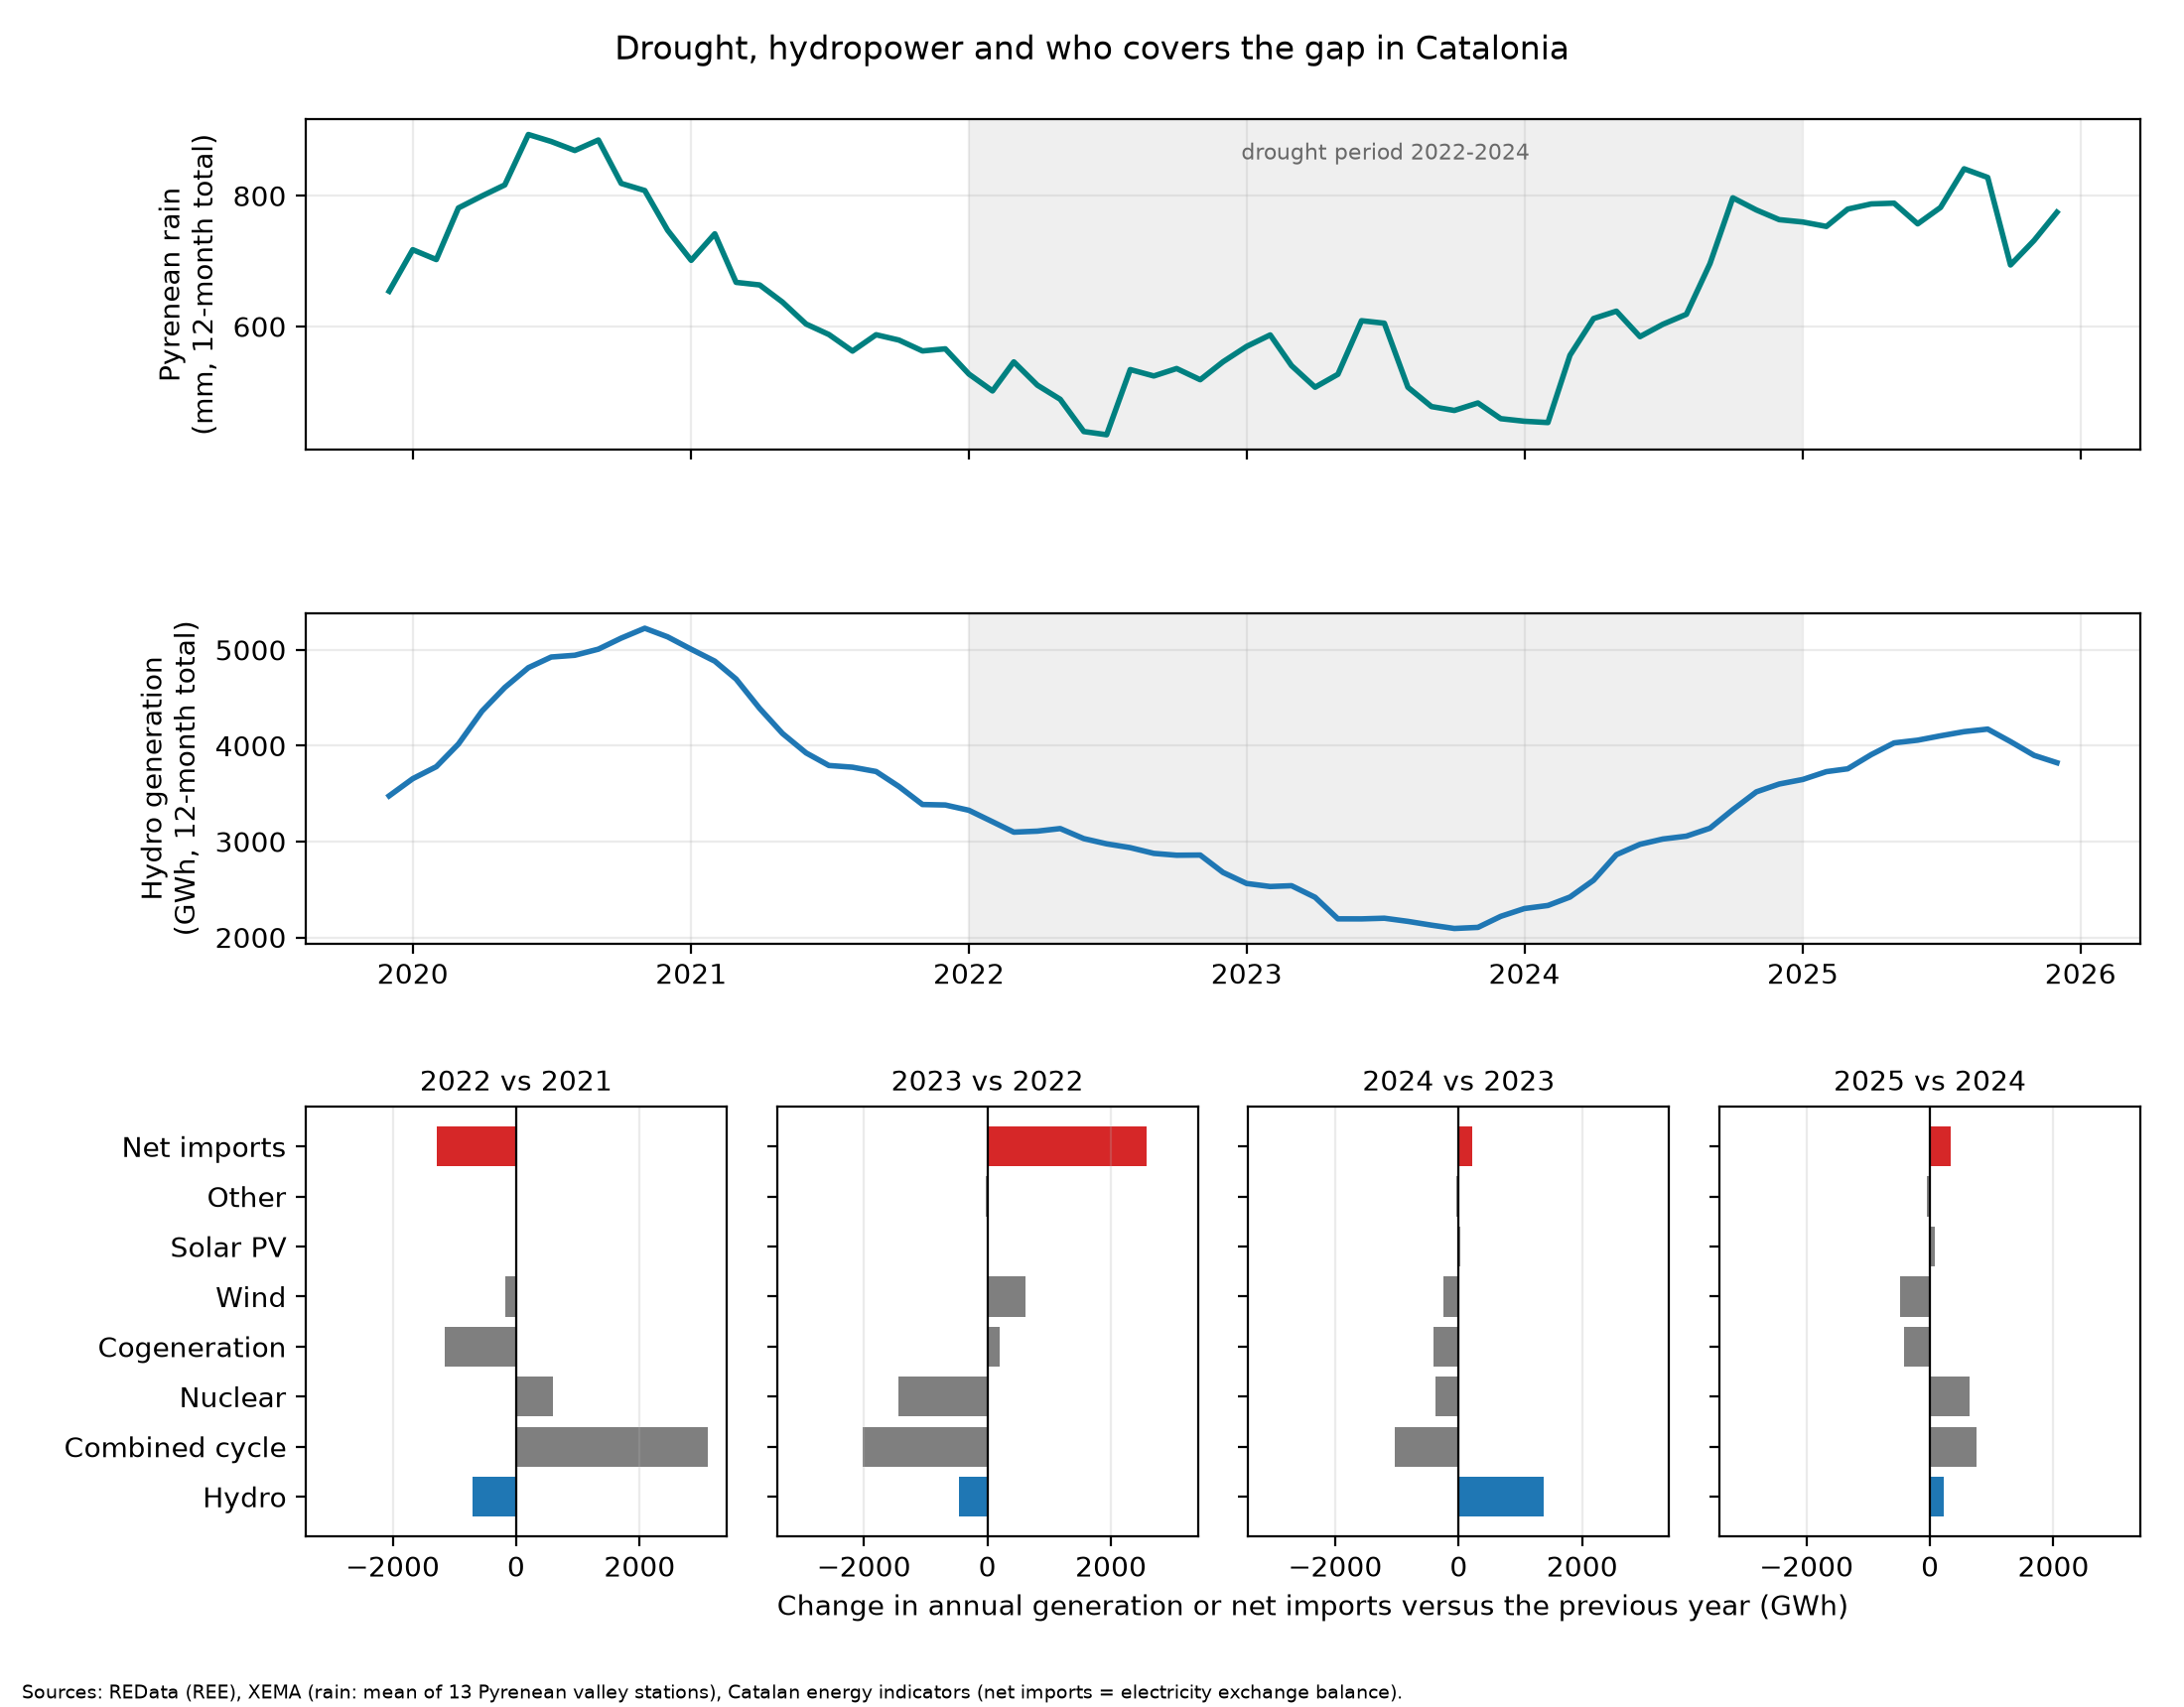
\includegraphics[width=0.8\linewidth]{idea6_hydro_drought_replacement.png}
\caption{\textbf{Hydropower follows Pyrenean rain, and imports filled the 2023 gap.} (a) Pyrenean rain and hydropower (12-month totals) and the volume of the Conques Internes reservoirs, each as a percentage of its own 2019--2025 mean; the shaded band is the 2022--2024 drought. (b) Change in generation by source and in net imports from 2022 to 2023 (GWh); the bars add up to the change in total supply (black). Hydropower in blue, net imports in red. The main values are in the 2023 column of Table~\ref{tab:changes}.}
\label{fig:hydro}
\end{figure}

\subsection{Olive oil: dry years raise prices, but weakly}

The olive oil CPI rose by 54.6\% in the year to December 2023, and its annual change peaked at 73.5\% in October 2023. The price index (2021\,=\,100) reached 265 in April 2024 and then fell. The four driest hydrological years in Andalusia are 2005, 2012, 2019 and 2023. Prices rose by 26.5\%, 18.0\%, fell by 11.4\% and rose by 54.6\% in those years, so three of the four went with a price rise. Other large rises (2015, 2021 and 2022) came with only mild rain deficits.

Across the 23 years from 2003 to 2025 the correlation between rain and the December price change is $r=-0.42$ for Andalusia ($p=0.047$) and $r=-0.31$ for Catalonia ($p=0.15$; Figure~\ref{fig:olive}). The rank correlations are weaker ($-0.33$ and $-0.15$), and neither is significant. Monthly lagged correlations give the same message: the strongest value for olive oil is $-0.35$ at a lag of 7 months with Andalusian rain, and $-0.29$ at 3 months with Catalan rain. Fresh fruit and vegetables show no clearer pattern. \textbf{H3} therefore holds in direction: Andalusian rain tracks the price a little better than Catalan rain. But the evidence is borderline, and a single measure of rain in two regions cannot capture what sets the price of olive oil, such as the size of the harvest, stocks and international markets.

\begin{figure}[t]
\centering
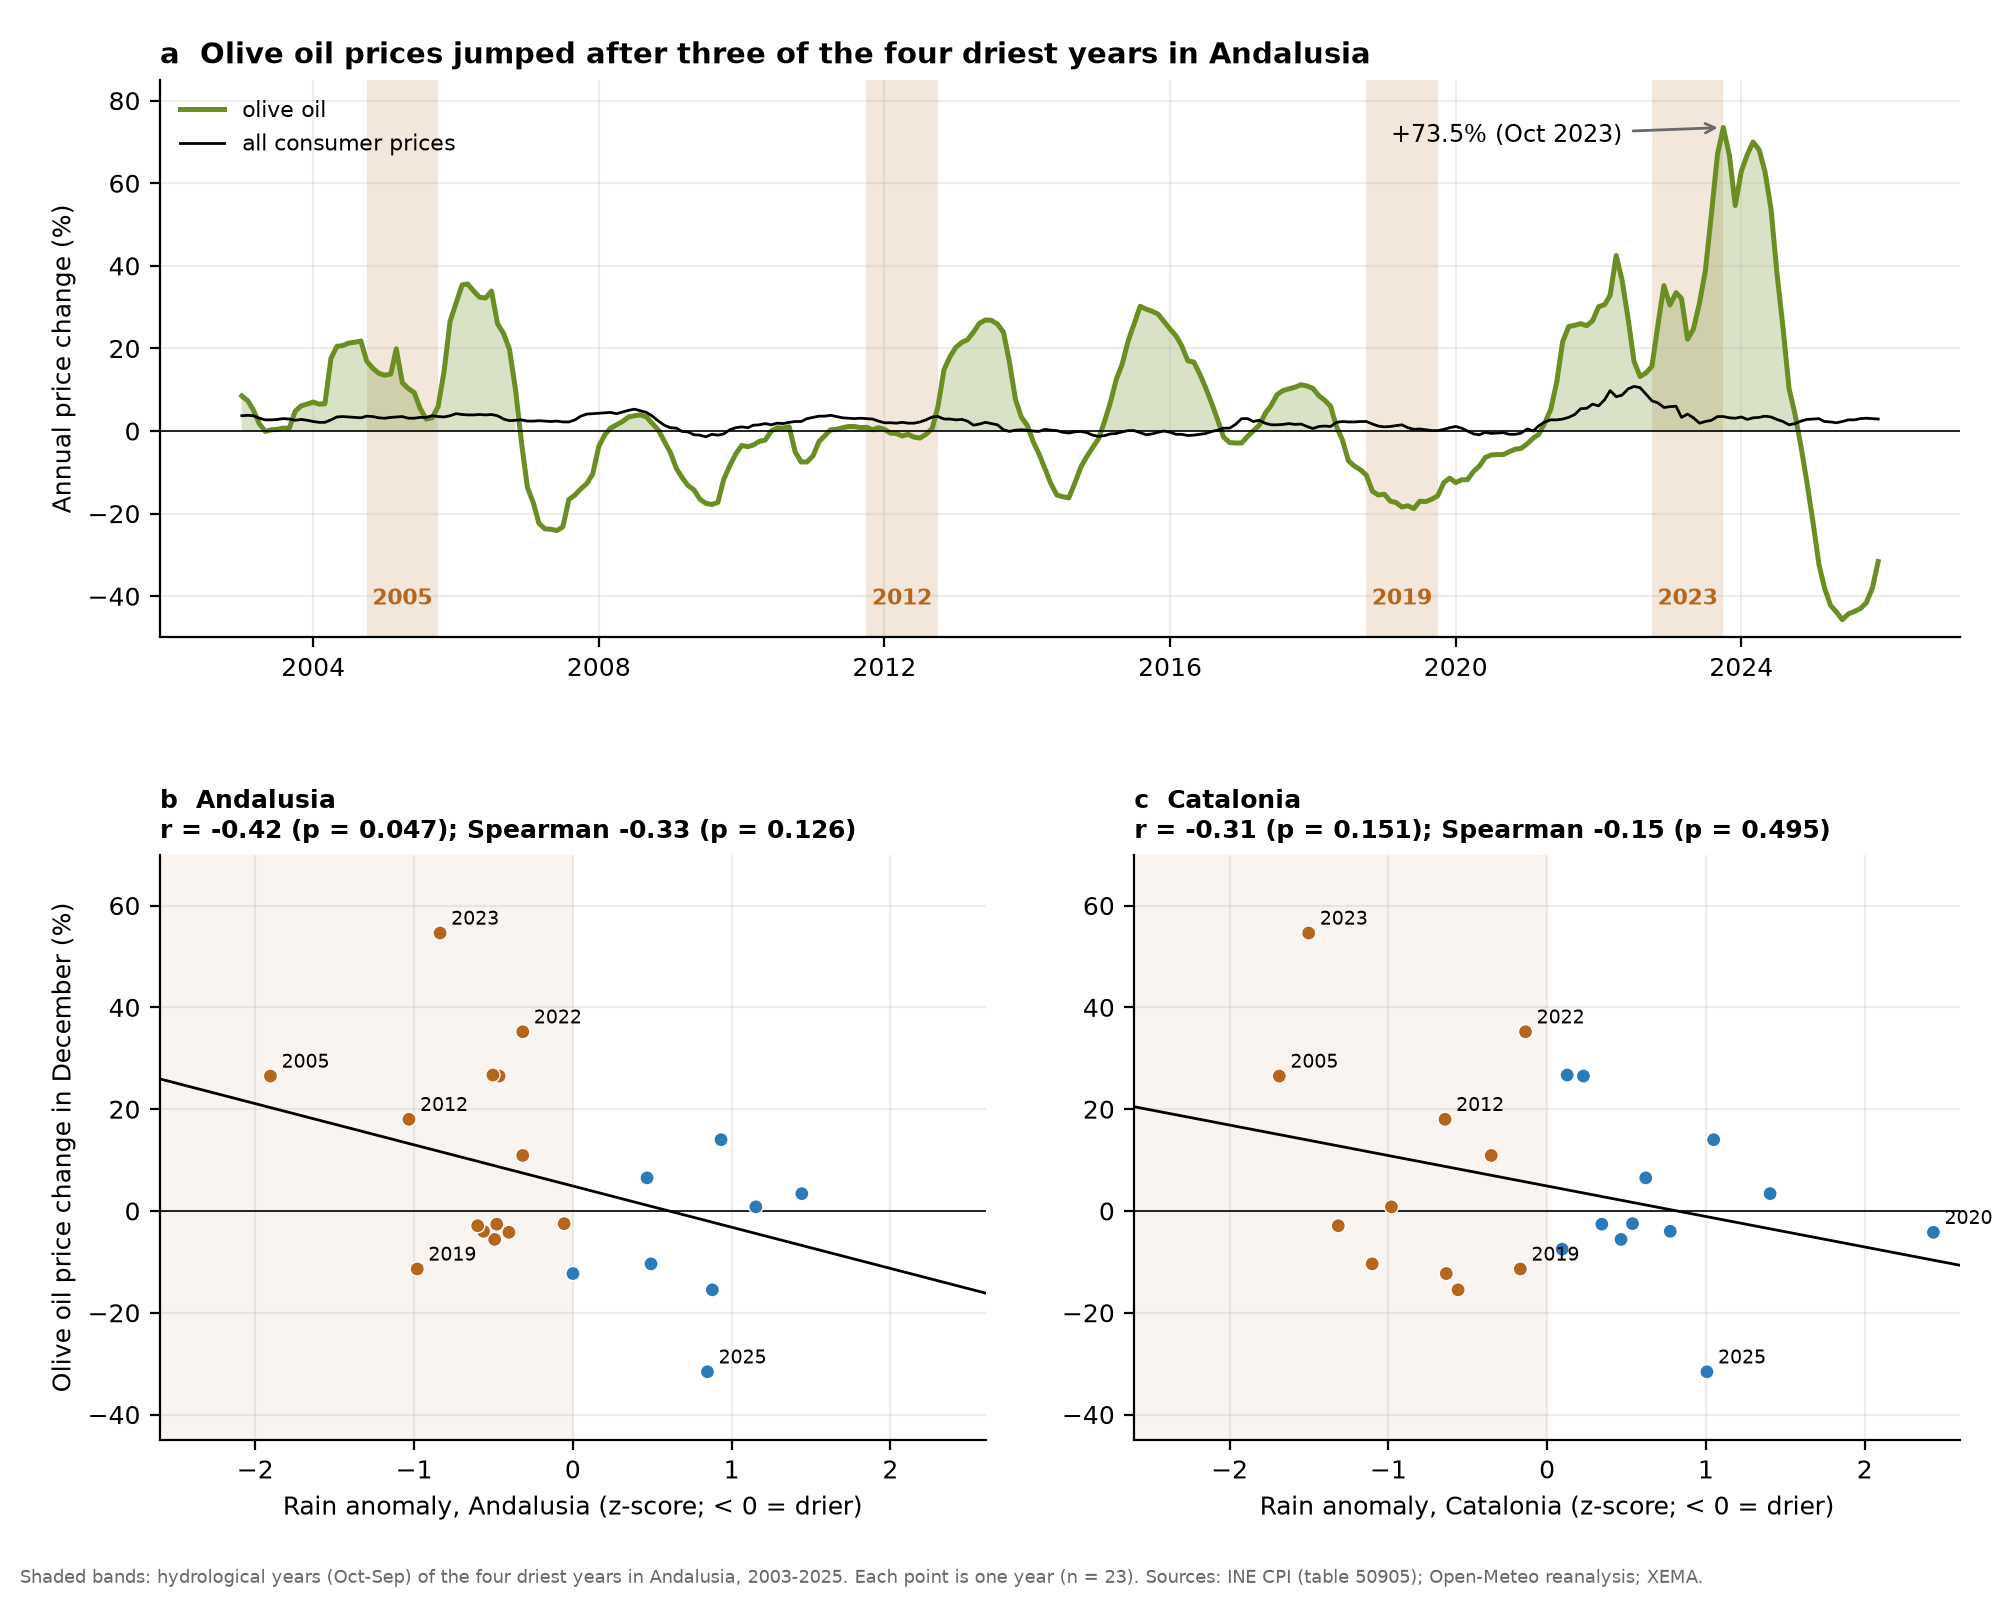
\includegraphics[width=0.82\linewidth]{idea4_olive_timeline.png}
\caption{\textbf{Dry years tend to raise olive oil prices, but the link is weak.} (a) Annual change of the olive oil CPI and of the general CPI; shaded bands mark the hydrological years of the four driest years in Andalusia. (b, c) Each point is one year (2003--2025): rain anomaly of the hydrological year against the change of the olive oil CPI in December, with the least-squares line, for Andalusia and Catalonia.}
\label{fig:olive}
\end{figure}

\subsection{Climate shelters in Barcelona: access is not the problem}

Barcelona has 564 climate shelters in the network we analysed. They include covered pools, libraries, nursery school yards, water play areas and civic centres, so they are not all equivalent (Figure~\ref{fig:map}). Across the city, 96.6\% of residents live within 400\,m of a shelter and 99.5\% within 800\,m. This agrees with the municipal claim that 99\% of the population has a shelter within 10 minutes on foot, at least in a straight line. Residents aged 75 or older do equally well (96.8\% and 99.6\%).

\textbf{H4} is not supported. The lowest-income decile has 97\% of its residents within 400\,m and all of them within 800\,m, and the correlation between income and distance to the nearest shelter is almost zero (Spearman $+0.07$). The weakest coverage is in the richest decile: 88.3\% within 400\,m and 98.6\% within 800\,m (Figure~\ref{fig:access}). This decile is 63\% Sarri\`a--Sant Gervasi and 11\% Les Corts. These areas are less dense, with a median of about 22\,700 inhabitants per km$^2$ against 38\,000--50\,000 in the other deciles, and their census sections are larger.

\begin{figure}[t]
\centering
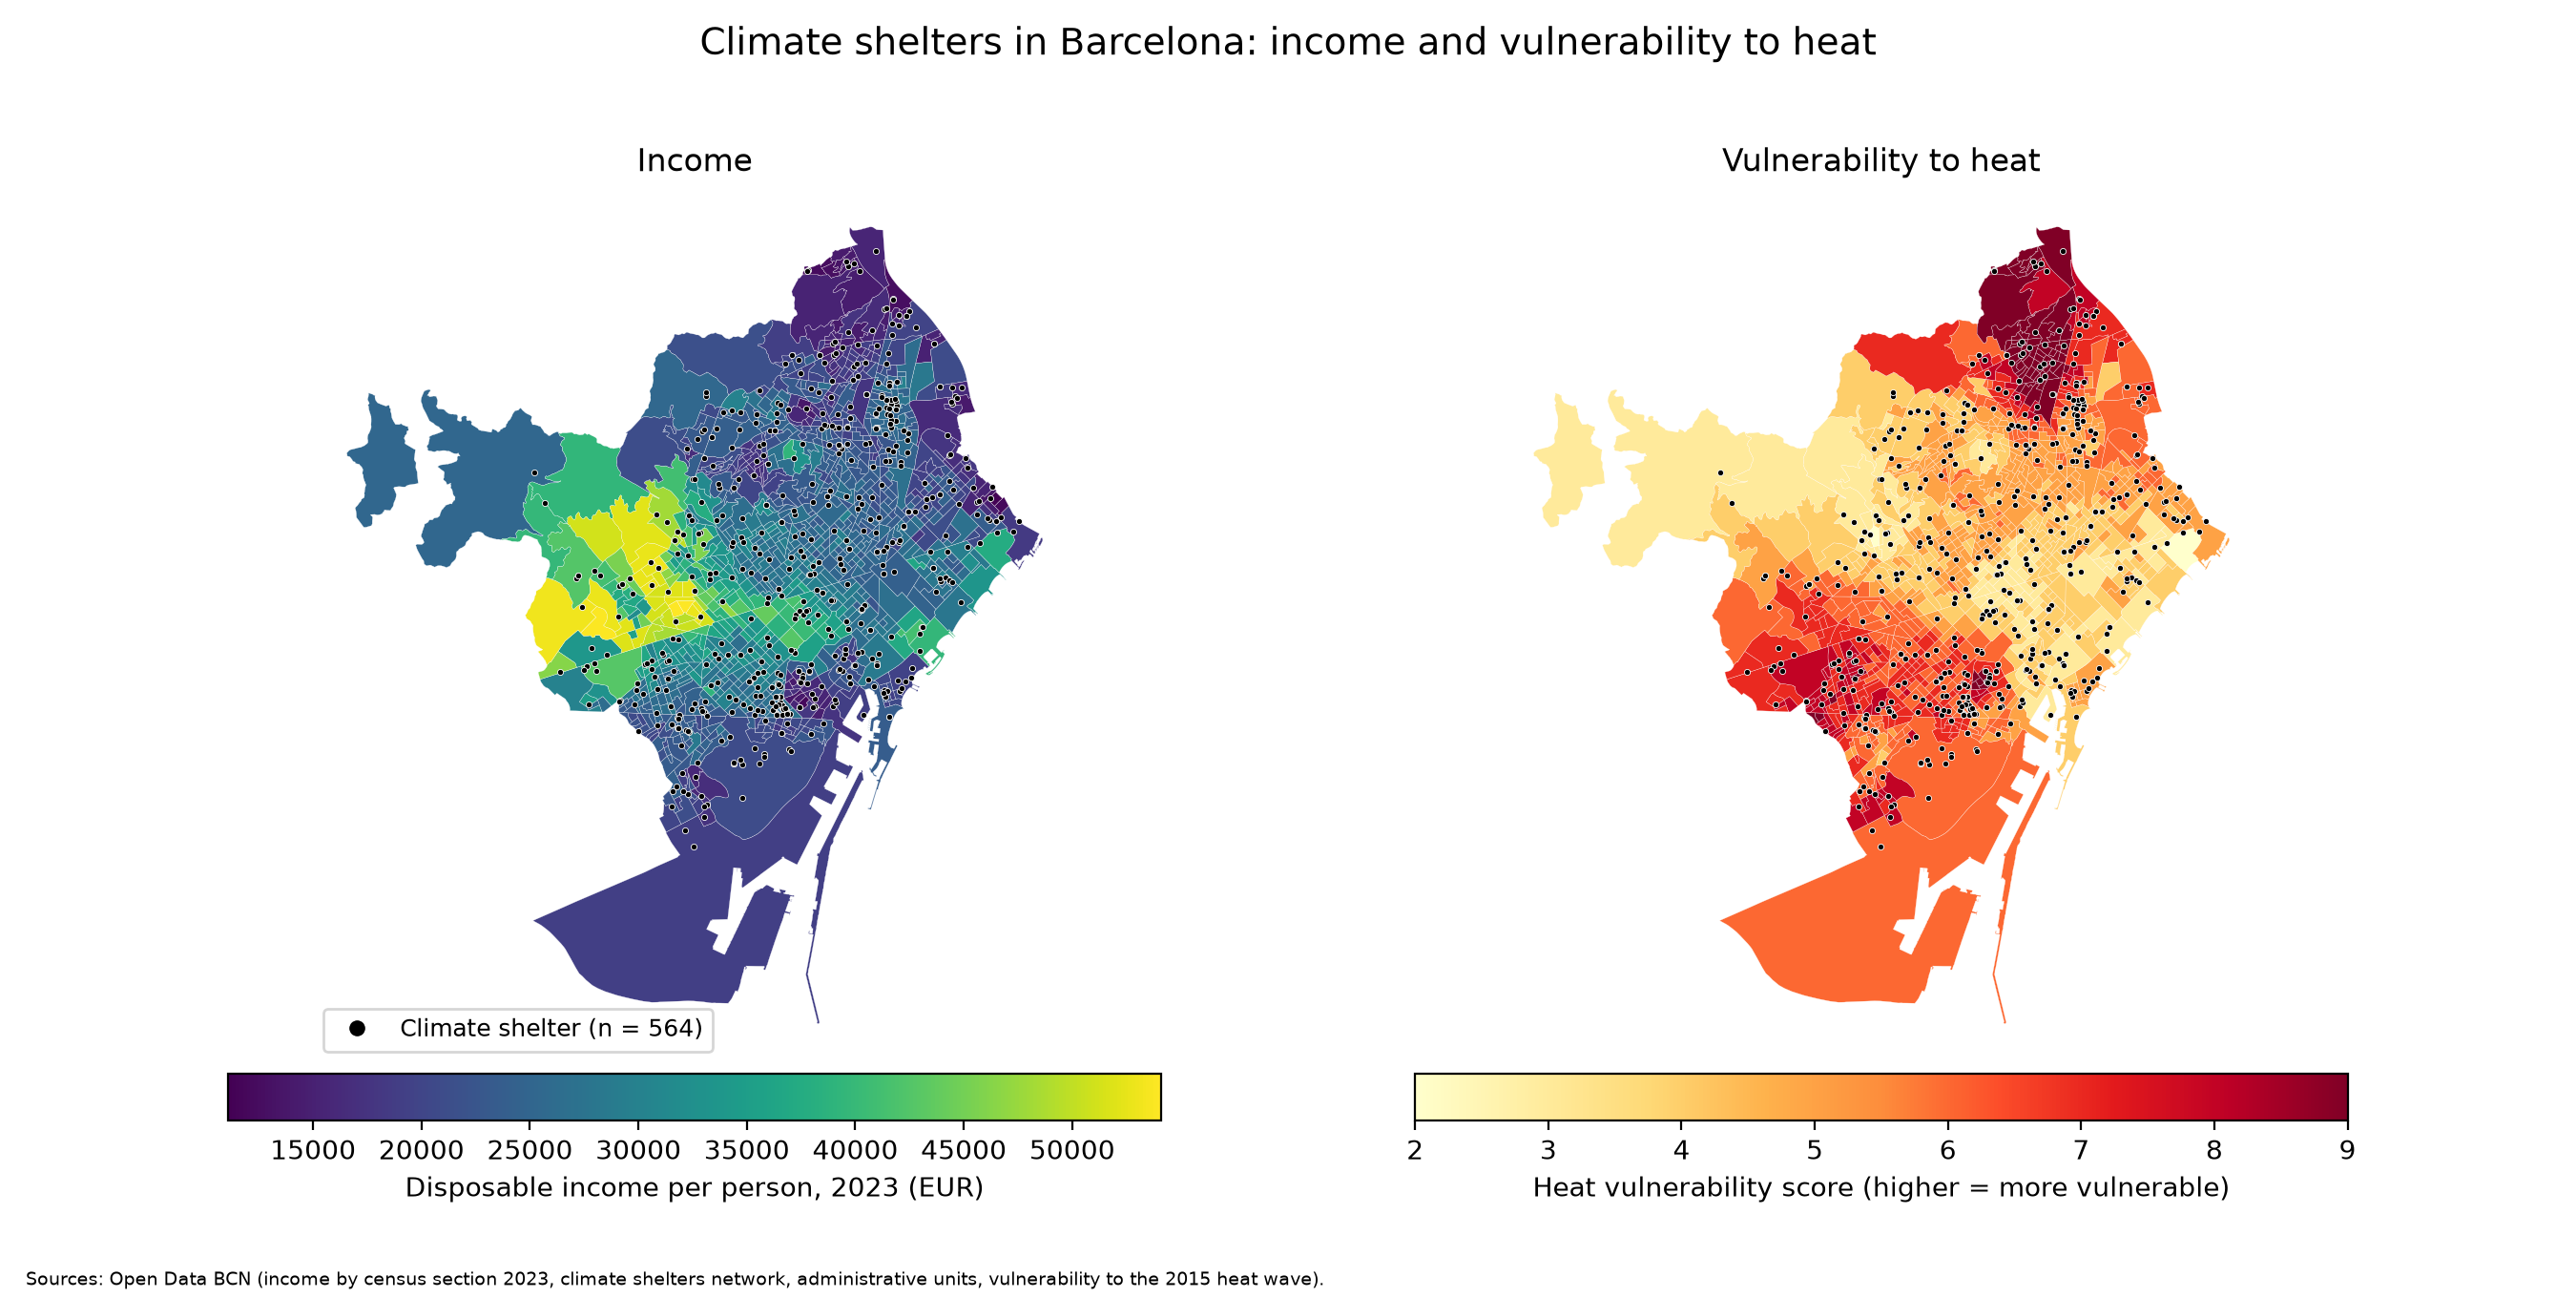
\includegraphics[width=\linewidth]{idea2_income_shelters_map.png}
\caption{Income per person (left) and vulnerability to heat (right) by census section in Barcelona. Black dots are the 564 climate shelters.}
\label{fig:map}
\end{figure}

\begin{figure}[t]
\centering
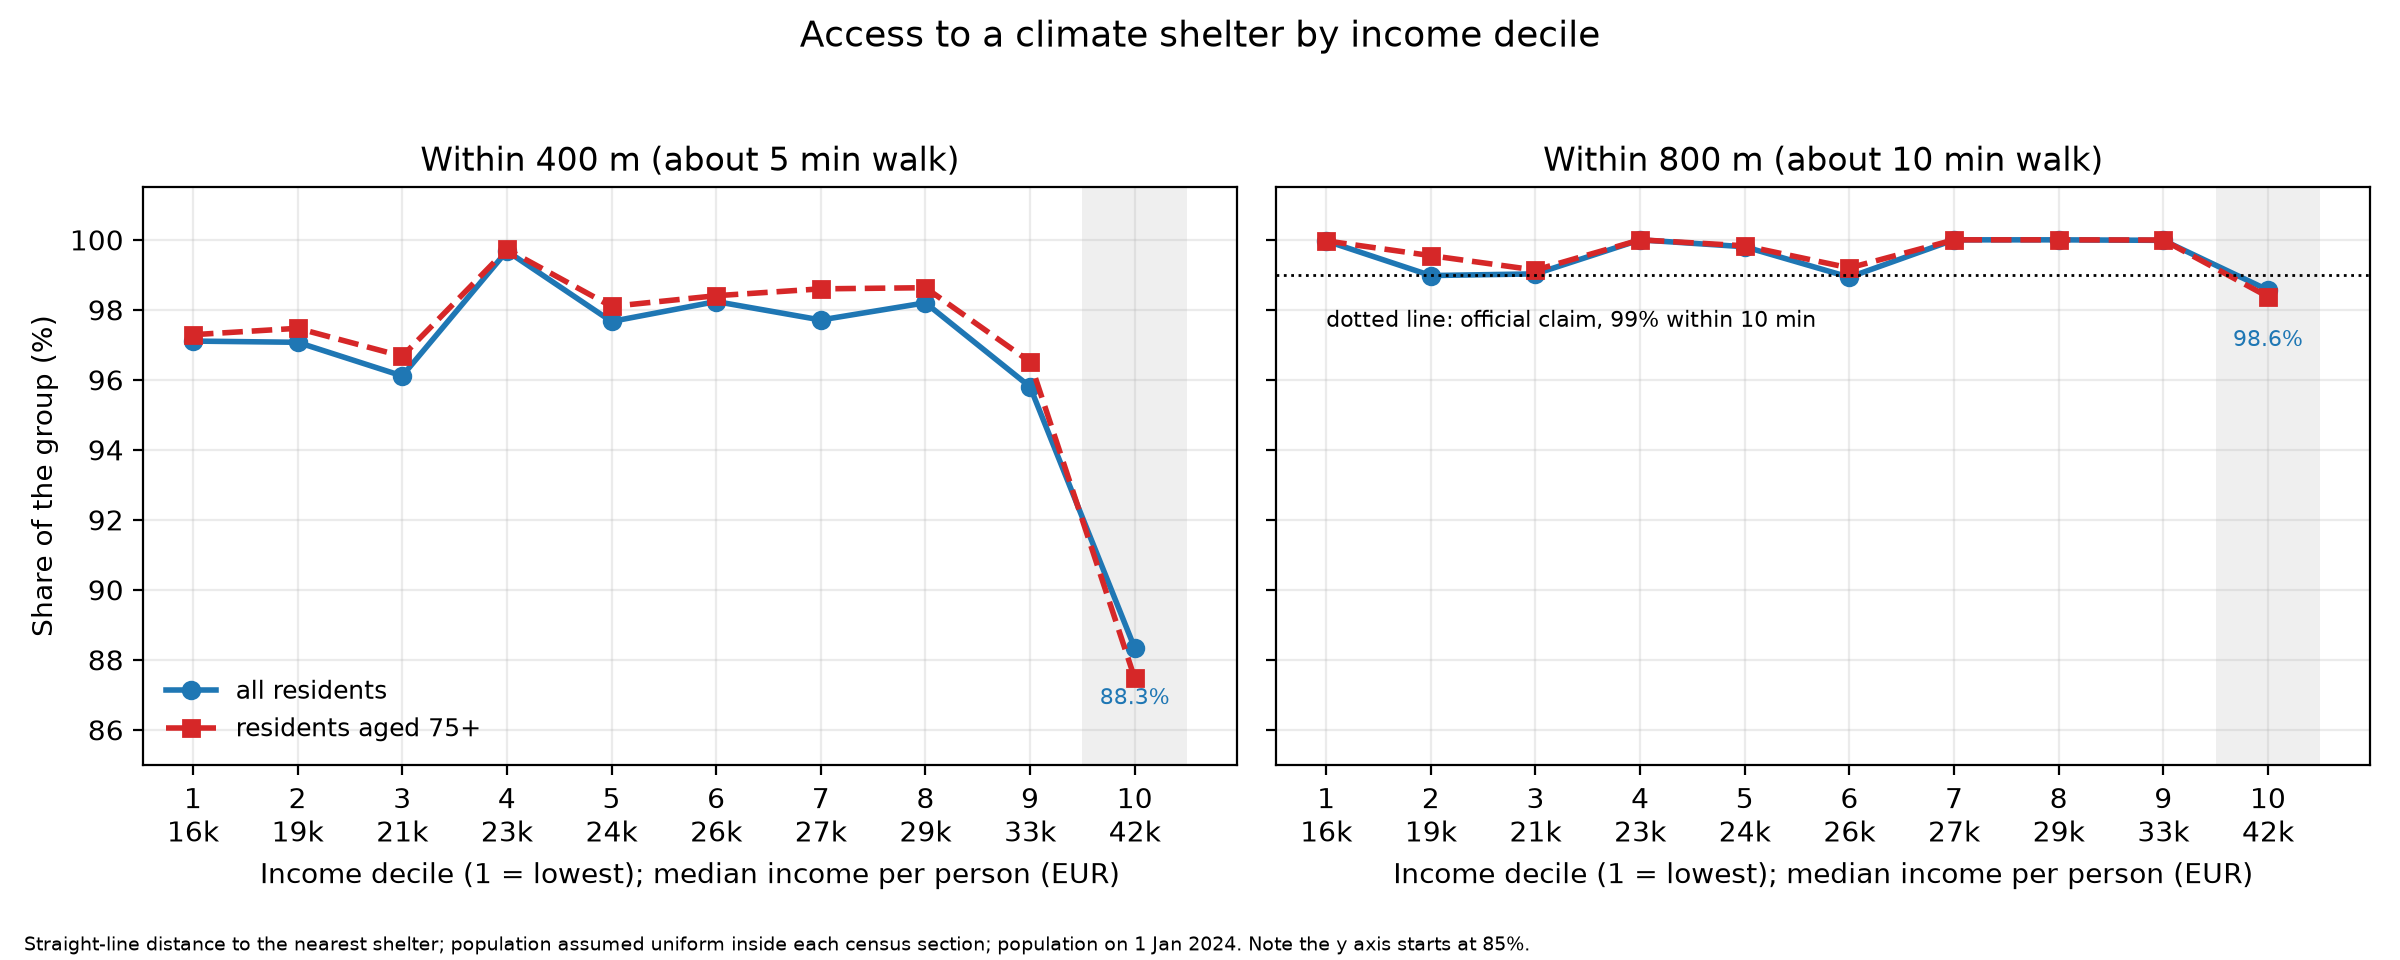
\includegraphics[width=0.78\linewidth]{idea2_accessibility_by_income.png}
\caption{\textbf{Access to shelters is almost the same in every income decile.} Share of residents within 400\,m (dark) and 800\,m (light) of a shelter, by income decile, on a full 0--100\% axis. The dashed line is the municipal claim of 99\% within 10 minutes. Only the richest decile falls clearly below it at 400\,m.}
\label{fig:access}
\end{figure}

The vulnerability score points the same way. It is highest in the poorest decile (7.2 on average, against about 5.0 in the upper half) and the shelters follow it. In sections with a high score there are 7.3 shelters per km$^2$, against 4.3 where the score is low (Figure~\ref{fig:vuln}). Part of this gradient comes from population density: per 10\,000 residents the numbers are almost equal (3.3 against 3.1). Coverage within 800\,m is 99.0\%, 99.7\% and 99.8\% in the low, medium and high classes. By this measure, the network does not under-serve the most vulnerable sections.

\begin{figure}[t]
\centering
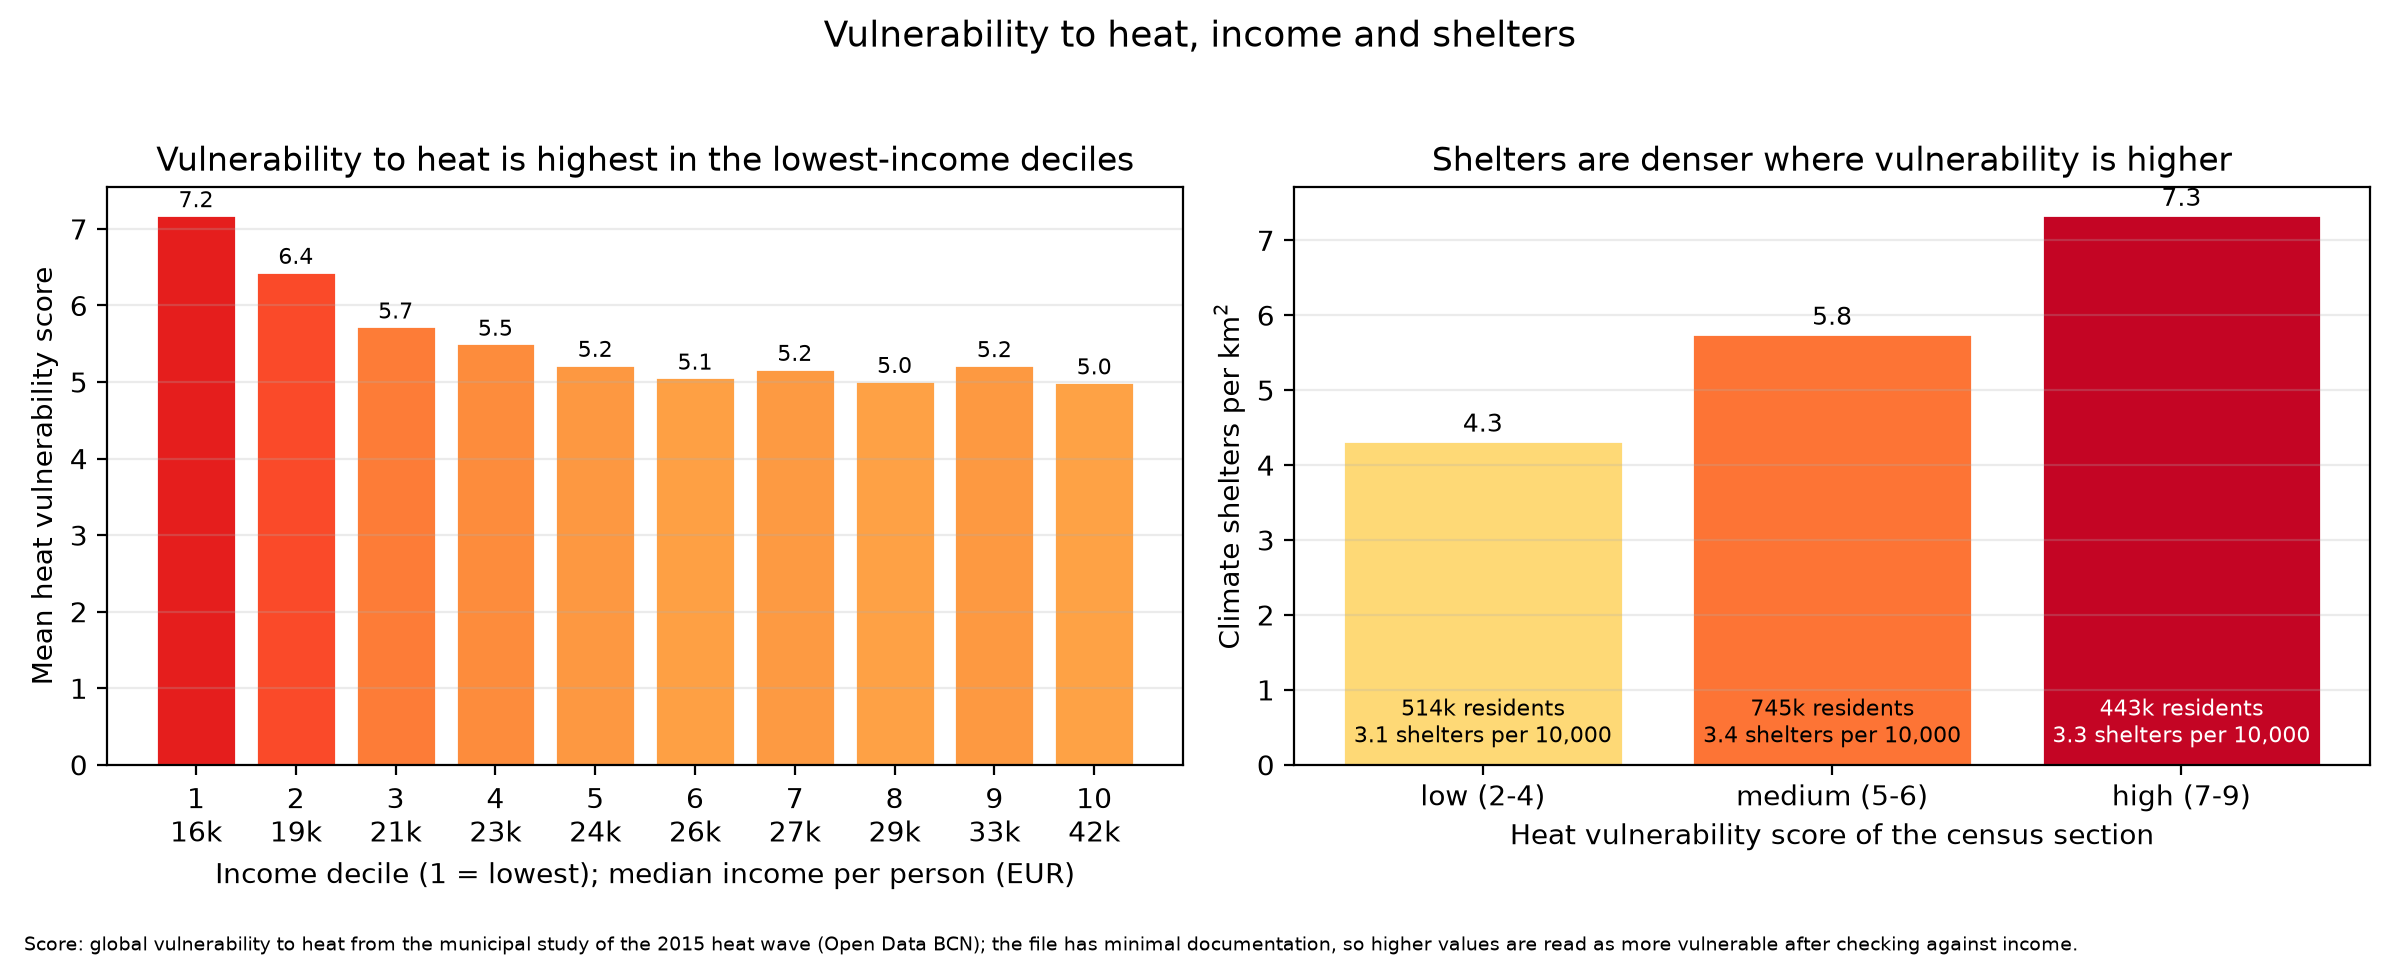
\includegraphics[width=\linewidth]{idea2_heat_vulnerability_by_income.png}
\caption{Left: mean vulnerability score by income decile. Right: shelters per km$^2$ by vulnerability class of the census section, with residents and shelters per 10\,000 residents of each class.}
\label{fig:vuln}
\end{figure}

\section{Discussion}

Three of the four expectations failed, and the failures are informative. Heat, not cold, makes demand rise faster (H1). Hydropower depends on rain in the Pyrenees, a different place from the reservoirs we used to look for the signal (H2). Access to shelters does not depend on income at the scale of walking distance (H4). The one expectation that held (H3) is also the least certain.

Several limits apply. All results are correlations, and the series are short: 912 days, seven years or 23 years, depending on the question. Rain is a proxy for drought, and for the harvest in particular it is a weak one. The Andalusian rain comes from a reanalysis grid and not from weather stations. In Barcelona we used straight-line distance, which understates the real walk along streets, and we assumed that residents are spread evenly inside each section, which penalises sections with parks or hillsides. The vulnerability score comes from a study of the 2015 heat wave, and the file has almost no documentation. We read higher values as more vulnerable because they are higher in lower-income sections and in the poorest hillside areas, and lower in the green districts. Finally, access is not exposure. We did not measure temperature inside the city, we did not consider opening hours or capacity of the shelters, and we compared income from 2023 with a vulnerability study from 2015.

\section{Conclusions}

Catalan electricity demand rises about 4.2\,GWh per day for each degree above 22\,$^\circ$C and 2.9\,GWh for each degree below 17\,$^\circ$C. The 2022--2024 drought lowered hydropower, but the gap was filled mostly by imports, and the reservoirs near Barcelona are a poor guide to hydropower, which follows Pyrenean rain. Dry years are linked to higher olive oil prices, but only weakly. In Barcelona, climate shelters are within reach of almost everyone, and their coverage does not fall with income. The natural next steps are walking distances along streets, measured temperatures in the city, and harvest data for olive oil.

\section*{Data and code availability}
The data are open (Table~\ref{tab:data}). The code, the notebooks and all figures are in the project repository: \url{https://github.com/NuriaMayoral/XEMAS-} (notebooks \texttt{gabri\_idea6}, \texttt{gabri\_idea4} and \texttt{gabri\_idea2}; figures in \texttt{figures/Gabri}).

\section*{Use of AI tools}
The analysis code, the figures and a first draft of this text were prepared with the help of Claude Code (Anthropic). The author reviewed the code, checked the numbers against known values and the original sources, and takes responsibility for the content. A log of the AI use is kept in the repository of the course.

\bibliographystyle{plainnat}
\bibliography{refs}

\end{document}
